
\section{Zehnerpotenzen}
\label{section:zehnerpotenzen}
\begin{frame}%STARTCONTENT

\frametitle{Große und kleine Werte}
\begin{itemize}
  \item Im Amateurfunk haben wir große und kleine Werte
  \item Um sich viele 0-en zu sparen, wurde bereits mit Einheitenvorsätzen abgekürzt, z.B. mit Milli (m) oder Kilo (k)
  \end{itemize}
\end{frame}

\begin{frame}
\frametitle{Zehnerpotenzen}
\begin{itemize}
  \item Einheitenvorsätze lassen sich in den meisten Taschenrechnern nicht direkt eingeben
  \item Stattdessen wird die Zehnerpotenz verwendet
  \item Kilo entspricht 1000 oder 10 $\cdot$ 10 $\cdot$ 10
  \item Abgekürzt 10<sup>3</sup>
  \end{itemize}
    \pause
    \qty{1500}{\hertz} $\rightarrow$ 1,5 kHz $\rightarrow$ 1,5 $\cdot$ 10<sup>3</sup> Hz

\qty{1500000}{\hertz} $\rightarrow$ \qty{1,5}{\mega\hertz} $\rightarrow$ 1,5 $\cdot$ 10<sup>6</sup> Hz

\end{frame}

\begin{frame}\begin{itemize}
  \item Milli entspricht  $\frac{1}{1000}$ oder $\frac{1}{10 \cdot 10 \cdot 10}$
  \item Abgekürzt 10<sup>-3</sup>
  \end{itemize}
    \pause
    \qty{0,0035}{\volt} $\rightarrow$ \qty{3,5}{\milli\volt} $\rightarrow$ 3,5 $\cdot$ 10<sup>-3</sup> V



\end{frame}

\begin{frame}
\frametitle{Einheitenvorsätze und Zehnerpotenzen}
\begin{table}
\begin{DARCtabular}{ccl}
     Bezeichnung  & Abkürzung  & Wert   \\
     Pico  & p  & 10<sup>-12</sup> = 0,000000000001   \\
     Nano  & n  & 10<sup>-9</sup> = 0,000000001   \\
     Mikro  & µ  & 10<sup>-6</sup> = 0,000001   \\
     Milli  & m  & 10<sup>-3</sup> = 0,001   \\
      &   & 10<sup>0</sup> = 1   \\
     Kilo  & k  & 10<sup>3</sup> = 1000   \\
     Mega  & M  & 10<sup>6</sup> = 1000000   \\
     Giga  & G  & 10<sup>9</sup> = 1000000000   \\
\end{DARCtabular}
\caption{Einheitenvorsätze für Zehnerpotenzen}
\label{e_einheitenvorzeichen}
\end{table}
\end{frame}

\begin{frame}
\frametitle{Taschenrechner}
\begin{columns}
    \begin{column}{0.48\textwidth}
    \begin{itemize}
  \item Taste \emph{EXP} oder \emph{$\cdot$10<sup>x</sup>}
  \item Eintippen: \enquote{145,3 Exp 6}
  \item Taste \emph{ENG} verschiebt den Exponent um 3
  \end{itemize}

    \end{column}
   \begin{column}{0.48\textwidth}
       
\begin{figure}
    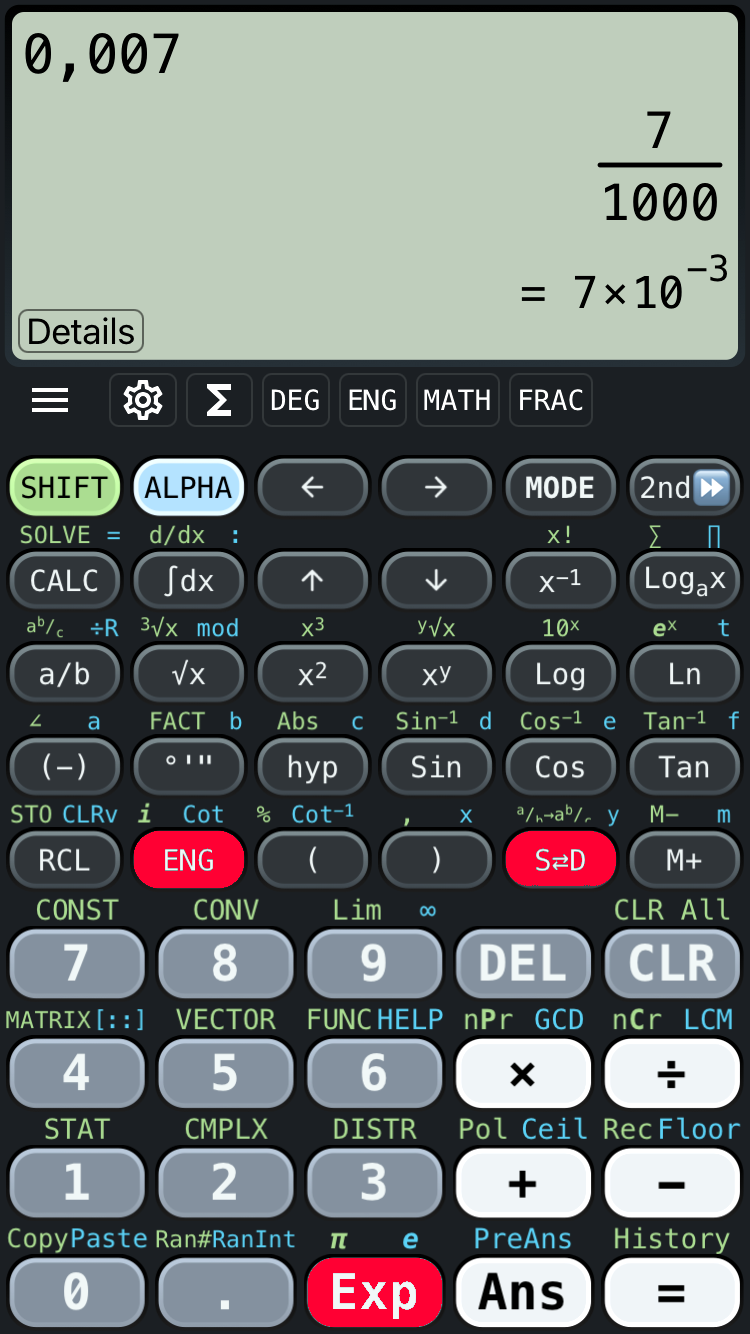
\includegraphics[width=0.85\textwidth]{foto/172}
    \caption{\scriptsize Verschiedene Darstellungen der Zahl 0,007 in einer Taschenrechner-App}
    \label{e_taschenrechner}
\end{figure}

   \end{column}
\end{columns}

\end{frame}

\begin{frame}
\only<1>{
\begin{QQuestion}{EA108}{\qty{0,00042}{\A} entspricht~...}{$420\cdot 10^6$ A.}
{$420\cdot 10^{-6}$ A.}
{$420\cdot 10^{-5}$ A.}
{$42\cdot 10^{-6}$ A.}
\end{QQuestion}

}
\only<2>{
\begin{QQuestion}{EA108}{\qty{0,00042}{\A} entspricht~...}{$420\cdot 10^6$ A.}
{\textbf{\textcolor{DARCgreen}{$420\cdot 10^{-6}$ A.}}}
{$420\cdot 10^{-5}$ A.}
{$42\cdot 10^{-6}$ A.}
\end{QQuestion}

}
\end{frame}

\begin{frame}
\only<1>{
\begin{QQuestion}{EA109}{\qty{0,042}{\A} entspricht~...}{$42\cdot 10^{-1}$ A.}
{$42\cdot 10^3$ A.}
{$42\cdot 10^{-2}$ A.}
{$42\cdot 10^{-3}$ A.}
\end{QQuestion}

}
\only<2>{
\begin{QQuestion}{EA109}{\qty{0,042}{\A} entspricht~...}{$42\cdot 10^{-1}$ A.}
{$42\cdot 10^3$ A.}
{$42\cdot 10^{-2}$ A.}
{\textbf{\textcolor{DARCgreen}{$42\cdot 10^{-3}$ A.}}}
\end{QQuestion}

}
\end{frame}

\begin{frame}
\only<1>{
\begin{QQuestion}{EA110}{\qty{4200000}{\Hz} entspricht~...}{$4,2\cdot 10^5$ Hz.}
{$4,2\cdot 10^6$ Hz.}
{$42\cdot 10^6$ Hz.}
{$42\cdot 10^{-5}$ Hz.}
\end{QQuestion}

}
\only<2>{
\begin{QQuestion}{EA110}{\qty{4200000}{\Hz} entspricht~...}{$4,2\cdot 10^5$ Hz.}
{\textbf{\textcolor{DARCgreen}{$4,2\cdot 10^6$ Hz.}}}
{$42\cdot 10^6$ Hz.}
{$42\cdot 10^{-5}$ Hz.}
\end{QQuestion}

}
\end{frame}

\begin{frame}
\only<1>{
\begin{QQuestion}{EA111}{\qty{0,01}{\mV} entspricht~...}{$1\cdot 10^{-7}$ V.}
{$10\cdot 10^{-6}$ V.}
{$10\cdot 10^{-5}$ V.}
{$0{,}01\cdot 10^{3}$ V.}
\end{QQuestion}

}
\only<2>{
\begin{QQuestion}{EA111}{\qty{0,01}{\mV} entspricht~...}{$1\cdot 10^{-7}$ V.}
{\textbf{\textcolor{DARCgreen}{$10\cdot 10^{-6}$ V.}}}
{$10\cdot 10^{-5}$ V.}
{$0{,}01\cdot 10^{3}$ V.}
\end{QQuestion}

}
\end{frame}

\begin{frame}
\only<1>{
\begin{QQuestion}{EA112}{\qty{0,002}{\Mohm} entspricht~...}{$20\cdot 10^{3} \Omega$.}
{$2\cdot 10^{3} \Omega$.}
{$2\cdot 10^{2} \Omega$.}
{$2000\cdot 10^{2} \Omega$.}
\end{QQuestion}

}
\only<2>{
\begin{QQuestion}{EA112}{\qty{0,002}{\Mohm} entspricht~...}{$20\cdot 10^{3} \Omega$.}
{\textbf{\textcolor{DARCgreen}{$2\cdot 10^{3} \Omega$.}}}
{$2\cdot 10^{2} \Omega$.}
{$2000\cdot 10^{2} \Omega$.}
\end{QQuestion}

}
\end{frame}

\begin{frame}
\only<1>{
\begin{QQuestion}{EA113}{$2\cdot 10^{-7}$ W entspricht~...}{\qty{20}{\micro\W}.}
{\qty{2}{\micro\W}.}
{\qty{0,2}{\micro\W}.}
{\qty{200}{\micro\W}.}
\end{QQuestion}

}
\only<2>{
\begin{QQuestion}{EA113}{$2\cdot 10^{-7}$ W entspricht~...}{\qty{20}{\micro\W}.}
{\qty{2}{\micro\W}.}
{\textbf{\textcolor{DARCgreen}{\qty{0,2}{\micro\W}.}}}
{\qty{200}{\micro\W}.}
\end{QQuestion}

}
\end{frame}

\begin{frame}
\only<1>{
\begin{QQuestion}{EA114}{$5 \cdot 10^{-1}$ W entspricht~...}{\qty{500}{\mW}.}
{\qty{5}{\W}.}
{\qty{-500}{\mW}.}
{\qty{-5}{\W}.}
\end{QQuestion}

}
\only<2>{
\begin{QQuestion}{EA114}{$5 \cdot 10^{-1}$ W entspricht~...}{\textbf{\textcolor{DARCgreen}{\qty{500}{\mW}.}}}
{\qty{5}{\W}.}
{\qty{-500}{\mW}.}
{\qty{-5}{\W}.}
\end{QQuestion}

}
\end{frame}

\begin{frame}
\only<1>{
\begin{QQuestion}{EA115}{0,22~μF entspricht~...}{\qty{22}{\pF}.}
{\qty{22}{\nF}.}
{\qty{220}{\pF}.}
{\qty{220}{\nF}.}
\end{QQuestion}

}
\only<2>{
\begin{QQuestion}{EA115}{0,22~μF entspricht~...}{\qty{22}{\pF}.}
{\qty{22}{\nF}.}
{\qty{220}{\pF}.}
{\textbf{\textcolor{DARCgreen}{\qty{220}{\nF}.}}}
\end{QQuestion}

}
\end{frame}

\begin{frame}
\only<1>{
\begin{QQuestion}{EA116}{\qty{3750}{\kHz} entspricht~...}{\qty{37500000}{\Hz}.}
{\qty{3,750}{\MHz}.}
{\qty{0,03750}{\GHz}.}
{\qty{0,3750}{\GHz}.}
\end{QQuestion}

}
\only<2>{
\begin{QQuestion}{EA116}{\qty{3750}{\kHz} entspricht~...}{\qty{37500000}{\Hz}.}
{\textbf{\textcolor{DARCgreen}{\qty{3,750}{\MHz}.}}}
{\qty{0,03750}{\GHz}.}
{\qty{0,3750}{\GHz}.}
\end{QQuestion}

}
\end{frame}%ENDCONTENT
